
% ----------------------------------------------------------------------------------------------------------------------
%     Node Histogram Distance
% ----------------------------------------------------------------------------------------------------------------------

\subsubsection{Node Histogram Distance}
\label{sec:Postprocessing:sub:DistanceMeasures:sub:NHD}

\todo{massen, die weit weg sind vom current node eines histogams sind auch weniger wichtig zu unterscheiden für diesen node.
i.e., je weiter weg, desto egaler ob die masse in dieser oder jener clade ist.
bei nahen massen ist der baum hingegen noch nicht so verzweigt, sprich, da hat man mehr genauigkeit/lokalität.
anders gesagt: je weiter weg, desto platter gebügelt werden die massen, weil mehr äste auf die selbe entfernung, dh das selbe bin gemappt werden}

\todo{lange dist ist auch in emd egal! 
approx with histogram, geht aber auch ohne, indem man ne double double map nimmt
}

We propose an alternative distance measure for phylogenetic samples, called the \emph{Node Histogram} (NH) distance.
\todo{Not sure whether it is a good idea to base the motivation solely on computational speed.
Maybe there is a better one.}
\alexis{das ist immer gut, wir brauchen halt nur beispiellaufzeiten hier um zu überezeugen dass das auch wirklich relevant ist}
It has similar properties as the KR distance, but offers some computational advantages.
Instead of moving placement masses on the \ac{RT} itself, the NH distance uses simple linear histograms
that describe the mass distribution.

The metric  is computed in two steps.
First, for each sample, a set of histograms is generated which describe its mass distribution.
Then, the histogram sets of two samples are used for calculating the pairwise distance.
Algorithm \ref{algo:NodeHistograms} illustrates how the histograms are computed.

\begin{algorithm}
\caption{Filling Node Histograms}\label{algo:NodeHistograms}
\begin{algorithmic}[1]
    \State $Histograms \gets \text{empty list}$
    \ForAll{$N \in \text{nodes of the tree}$}
        \State $H \gets \text{empty histogram}$
        \ForAll{$Q \in \text{queries of the sample}$}
            \ForAll{$P \in \text{placements of } Q$ }
                \State $d \gets \text{Distance}( P, N ) $
                \State $ H(d) \gets H(d) + \text{LWR}(P) $
            \EndFor
        \EndFor
        \State normalize $H$
        \State $Histograms(N) \gets H$
    \EndFor
    \State \textbf{return} $Histograms$
\end{algorithmic}
\end{algorithm}

The algorithm starts by creating a one-dimensional histogram for each node of the \ac{RT}.
% These histograms collect the placement masses of a sample.
The range of each histogram spans the longest distance (in branch length) from its node to any other node in the tree.
\todo{add the negative axis here if the test results show that this is a good extension.}
The number of histogram bins into which this range is divided is a hyper-parameter
that can be used to trade resolution for computational cost.
We used 25 bins per histogram, because ...
\todo{Need to add some test results here. Also, do some tests how the number of bins changes results}.
% The height of each bin represents the masses. %along the edges of the tree.
% so that it is able to capture the distribution of all mass points.
The histograms are then filled with all masses of the sample:
For each histogram and for each placement location of a \ac{QS}, the \ac{LWR} of that placement is added to the bin
that represents the distance from the placement location to the node of the histogram.
This is repeated for every \ac{QS} in the sample.
Lastly, the histograms are normalized, so that the sum of their bins is $1.0$.
In short, each histogram collects the distribution of placement masses as seen from its corresponding node.
The set of histograms for a sample then collectively describes its overall mass distribution
and implicitly captures the topology of its \ac{RT}.
Figure~\ref{fig:nhd} shows an example.

\begin{figure}[hpbt]
    \centering
    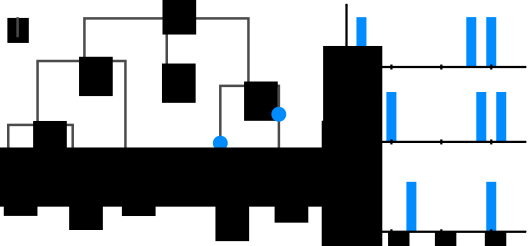
\includegraphics[width=\linewidth]{img/nhd.pdf}
    \caption{
        \textbf{Node Histogram Distance.}
        The left shows the reference tree with three placements of a sample.
        For simplicity, all of them are considered to have a mass of 1.0.
        The right shows exemplary histograms for the nodes \texttt{A}, \texttt{B} and \texttt{H}.
        They indicate how far the placement masses are located from the respective nodes.
        The same set of histograms is generated for other samples.
        The NH distance between two samples is then calculated
        using the average KR distance between corresponding pairs of node histograms of the samples.
    }
    \label{fig:nhd}
\end{figure}

% In order to then measure the distance between two samples, their histograms sets are used.
The second step then calculates the distance between two samples based on their histograms.
As both samples have been placed onto the same underlying \ac{RT}, their histograms form pairs corresponding to
the same \ac{RT} nodes.
For each node, the distance between two histograms is calculated using the KR distance,
that is, their distance is the minimum cost of turning one histogram into the other.
These distances are summed up over all nodes, and normalized by dividing by the number of nodes to calculate the average.
A further optional normalization step is to divide by the tree length,
which yields comparable distances across different \acp{RT}.

The main advantage of this method is its computational speed.
For current \ac{RT} sizes as well as sample sizes and numbers, it is still feasible to use the KR distance,
but dataset sizes will grow beyond that based on the current trend.
\todo{add compute times for some of the previously mentioned datasets here.}
Note that, the histograms for the NH distance have only to be computed once per sample,
and can be reused for subsequent distance calculations.
As they are linear, and combine nearby placements into the same bin,
histograms are much faster to process than a complex tree structure.
Particularly for calculating a pairwise distance matrix between samples,
which is needed for most subsequent methods,
this yields large speedups.
\alexis{also say something about the loss in accuracy, if any!}
\todo{Need to quantify! Run some tests!}

Furthermore, the calculation can be made even faster and more memory efficient by reducing the number of histograms,
e.g., by only generating them for leaf nodes. \alexis{how would that help, how much information.resolution would we lose?}
Finally, if the number of \acp{QS} become even too large for this,
it is possible to only use a subset of them to add their masses to the histograms.
This results in an anytime algorithm that yields a more accurate estimate of the distance the longer it runs,
but that can be stopped at any time.
\todo{Is this too far into the future? I think it's a neat property of the algorithm, but maybe too much to mention here...}
\alexis{I think the above paragraph should be ommitted}

\todo{Make NMDS plots comparing the distances matrices obtained from KR and ND distances, to show that they are similar.}

\todo{New idea: make the histograms also go into negative direction.
Use this extra space to distinguish between placements towards the root and away from the root,
as seen by the node to which the histogram belongs. Will try.}

\todo{More thoughts on NHD: it basically flattens the tree into 1D. with negative NHD histograms, we at least also use
a bit more resolution. but generally we can say that the distances approximates that tree by reducing the complexity of
the tree topology onto a line. furthermore, binning to a histogram makes it even more of an approximation.}

\todo{Even more thoughts: If I'm not mistaken, the NHD always underestimates the difference
(because the distances due to topology are all flattened into the 1D axis of the histograms),
i.e., it is always <= KR distance.
If that's the case, this could be mentioned here, along with some examples where they are the same,
and where they maximally differ. Maybe even proof this (if necessary).}
\alexis{the above sounds pretty cool :-) }

% ======================================================================================================================
%     Distance Measures
% ======================================================================================================================

\subsection{Distance Measures}
\label{sec:Evaluation:sub:DistanceMeasures}

accuracy nh vs kr distance, speed comparison, etc

speed test: parallelized version vs guppy, on play and on hitssv542

compare distance matrices of KR and NH distance using Mantel's test \cite{Mantel1967,Legendre1998}

% ======================================================================================================================
%     Simulated Data
% ======================================================================================================================

% \subsection{Simulated Data}
% \label{sec:Evaluation:sub:SimulatedData}
%
% \begin{itemize}
%     \item Three extreme tree shapes, comb-like, and fully balances, rooted and unrooted,
%     in order to evaluate the robustness/limits/workings of the clustering.
%     \item Show examples of trees with distributions.
%     \item Calculate NH distance, show MDS plots of the resulting distance matrix, in comparison to MDS plot using KR distance.
%     \item Also show clustering using k-means on that data. Can be visualized via color in the MDS plots,
%     or similar to HMP data, see below.
%     \item some speed comparisons: kr vs nhd, vs guppy implementation.
% \end{itemize}


% ----------------------------------------------------------------------------------------------------------------------
%     Binning
% ----------------------------------------------------------------------------------------------------------------------

\subsubsection{Binning}
\label{sec:Evaluation:sub:DistanceMeasures:sub:Binning}

speed tests, how much accuracy is lost etc

% ======================================================================================================================
%     Clustering
% ======================================================================================================================

\subsection{Clustering}
\label{sec:Postprocessing:sub:Clustering}

kmedians, pam, mds, … colour according to metadata

compare to edge pca

\url{http://stats.stackexchange.com/questions/183236/what-is-the-relation-between-k-means-clustering-and-pca}

\url{https://stats.stackexchange.com/questions/203766/use-cases-for-coefficient-of-variation-vs-index-of-dispersion/203808#203808}

4. Distance Calculation
emd, node histogram distance.


time for results! results results! :tada:
first: kmeans on trees. each sample (jplace file) is one data point to be clustered. using EMD as distance measure, and building centroids for each cluster by aggregating and normalizing the masses of the trees assigned to each cluster.
first test on the bacterial vaginosis data, because it is small and i can compare results to the BV paper.
using 3 clusters, because this seemed reasonable
as a reminder, here is the MDS plot (using EMD to build a pairwise distance matrix for all samples, then using mutidimesional scaling to fit this into a 2d picture)
we see that the blue blob in the right are the sick patients. the healthy red ones on the left are a bit spread out
this method finds sick patients, but is not further able to distinguish them. so far, nothing new

now the results of the clustering
the first picture (tree 0) corresponds to the blue blob of the MDS plot. we see two purple regions on the left of the tree, which belong to the clades "Lactobacillus iners" and "Lactobacillus crispatus", respectively - which are exactly the two clades that the EdgePCA method can distinguish, but EMD not (more on that later).
that means, the result of the EMD kmeans is exactly as expected from what we know about strengths and weaknesses of the EMD so far
the other two trees then correspond to patches of the red dots in the MDS plot - not much to explain here.
here are some number details about those cluster:

Cluster 0    116 Elements  Avg Nugent Score 1.94
Cluster 1    53 Elements   Avg Nugent Score 8.21
Cluster 2    51 Elements   Avg Nugent Score 7.84

the nugent score corresponds to the red/blue coloring in the MDS plot
so, after this already looked pretty nice and promising, i though, it must be possible to do kmeans using the EdgePCA data. so, i used this data (which is simply a matrix) and fed it into my normal euclidean kmeans

first, here is the EdgePCA plot as a reminder
now, the sick ones are one the left, separated into the two Lactobacillus groups

and here is the result of the kmeans clustering

Cluster 0    104 Elements    Avg Nugent Score 8.13
Cluster 1    73 Elements     Avg Nugent Score 2.84
Cluster 2    43 Elements     Avg Nugent Score 0.19

unfortunately, i have not yet figured out a way of visualizing this easily, because we are not dealing with trees any more. EDIT: not true. we are still dealing with trees. i can map back the matrix data onto edges. this should work. woah! (edited)
the table above basically says that cluster 0 now corresponds to the red dots (high nugent score), while clusters 1 and 2 are the blue dots (lower score) (edited)
also, as a mathematical remark, there is a connection between pca and kmeans: the normal vectors on the plane that the kmeans clusters span are the same as the first principal components
so, there is also a mathematical reason why the kmeans stuff works
so far for today. tomorrow, i'll prepare this whole thing for the big data sets. let's get hits106 to work for some time...

oh, one last addition to yesterday's results. @pierre.barbera  and i discussed the findings and also had another look at the BV paper. there, we find this figure
on the left hand side, it shows a cluster tree made via "squash clustering", which is a hierarchical method, i.e., it stepwise combines the closest two entities - in this case, using EMD as distance measure. (edited)
the bottom half (short branches in the cluster tree, red and orange in the taxonomic assigment) are the sick patiens, while the top half (longer branches, colorful tax assignment) are the healthy ones. (edited)
this is the same information as the first plot i posted last night (MDS using EMD): the sick ones get one close blue bubble, while the healthy ones are more spread out. (edited)
what that implies is that all those methods can basically be divided into two categories: using EMD as distance, and using edge imbalance as distance. then, MDS, PCA, Kmeans and squash clustering are just different ways to cluster/split/visualize this. which means, we can take the cross product of ( EMD | edge imbalance ) x ( MDS | PCA | Kmeans | squash clustering ) and end up with 8 different but similar methods :smile: (edited)
now we take the cross product of this with the >12 data analyses that i already have, and i am busy running jobs for the rest of my phd...

% ======================================================================================================================
%     Metagenomic Datasets
% ======================================================================================================================

\section{Metagenomic Datasets}
\label{sec:MetagenomicDatasets}

\begin{itemize}
    \item We used four datasets: BV, Neotrops, HMP and Tara.
    \item Download links etc
    \item Description of their features, num of reads, unique reads, etc
    \item Description of their metadata, maybe some examples.
\end{itemize}


\todo{refer to the number of total sequences as amplicons in the supplement. they are already deduplicated!}

\todo{add sample min max avg sizes (number of seqs per sample) to table}

%  Number of sequences per sample:
% tara
% min  11464
% max 811295
%
% bv
% min    506
% max  21426
%
% nts
% min     29
% max 290016
%
% hmp
% min      0
% max 403211


\todo{add references to data papers}

tara, hmp, bv, neotrops. individual pre-processing necessary.

what kind of data, how many samples, seqs, length hists, uniqs and duplicates.

% ----------------------------------------------------------------------------------------------------------------------
%     Bacterial Vaginosis
% ----------------------------------------------------------------------------------------------------------------------

\subsection{Bacterial Vaginosis}
\label{sec:MetagenomicDatasets:sub:BacterialVaginosis}

obtained the data from Sujatha Srinivasan and Erick Matsen. thanks again

uniq seqs: 15060
total seqs: 426612

seq len mean 226.2
seq len stddev 15.9

% ----------------------------------------------------------------------------------------------------------------------
%     Neotropical Soils
% ----------------------------------------------------------------------------------------------------------------------

\subsection{Neotropical Soils}
\label{sec:MetagenomicDatasets:sub:NeotropicalSoils}

% ----------------------------------------------------------------------------------------------------------------------
%     Tara Oceans
% ----------------------------------------------------------------------------------------------------------------------

\subsection{Tara Oceans}
\label{sec:MetagenomicDatasets:sub:TaraOceans}

\todo{check readme in sftp://czechls@magny-login/home/czechls/projects/data/tara}

Amplicon sequencing of Tara Oceans DNA samples corresponding to size fractions for protists.
% https://www.ebi.ac.uk/ena/data/view/PRJEB402

data from \href{https://www.ebi.ac.uk/ena/data/view/PRJEB6610}
on 2016-09-08

at the time of writing, 1170 samples were found...



only raw fastq files. used pear for paired end merging in order to get sequences.

used PEAR \cite{Zhang2014} to merge paired end reads.

370 samples with a total (unfilted) of 49,023,231 sequences.
filter out too short (<95) and too long (>150) seqs, just to be sure.
this removes x many, or y\% of the seqs.
samples: 370

uniq seqs: 27,697,007
chunks: 554

seq len mean 128.7
seq len stddev 11.4

we ran chimera detection. found x many.
compare to the ``bad'' placements where the lwr was low for all placements
(so that they were filtered out, causing the nasty broken jplace bug):
there are x many broken seqs, out of which y are also chimeric.

placement revealed some sequences with a very flat distribution, i.e., no proper ref sequence.
those might be chiemeric seqs. in order to find out, we used vsearch and swarm

\begin{verbatim}
Latitude Start
Longitude Start
Depth
Size Fraction Lower Threshold
Size Fraction Upper Threshold
Temperature
Salinity Sensor
Oxygen Sensor
Nitrate Sensor
Chlorophyll Sensor
\end{verbatim}

% ----------------------------------------------------------------------------------------------------------------------
%     Human Microbiome Project
% ----------------------------------------------------------------------------------------------------------------------

\subsection{Human Microbiome Project}
\label{sec:MetagenomicDatasets:sub:HumanMicrobiomeProject}

16S rRNA sequencing

start with 9811 samples, remove too big ones (> 70,000,000 bytes, 10 of them)

see sftp://czechls@magny-login/home/czechls/projects/data/hmp
for readme that explains all preprocessing

seq len mean 413.4
seq len stddev 143.6

filtered out everything between len ...

remove too short ones (< 1500 seqs), end up with 9194 samples

unfiltered number of sequences: 118,702,967

total seqs 118,701,818 ? according to length hist spreadsheet
samples: 9194

uniq seqs: 63,221,538
chunks: 1265

Body sites:

\begin{verbatim}
anterior_nares
attached keratinized_gingiva
attached_keratinized_gingiva
buccal_mucosa
hard_palate
left_antecubital_fossa
left_retroauricular_crease
mid_vagina
NA
palatine_tonsils
posterior_fornix
right_antecubital_fossa
right_retroauricular_crease
saliva
stool
subgingival_plaque
supragingival_plaque
throat
tongue_dorsum
vaginal_introitus
\end{verbatim}

see mapseq paper for hmp processing description


% ======================================================================================================================
%     Phylogenetic Placement
% ======================================================================================================================

\section{Phylogenetic Placement}
\label{sec:PhylogeneticPlacement}

\begin{itemize}
    \item de-duplication
    \item Prepare four datasets individually, so that we have a \texttt{fasta} file per sample.
    \item Our environmental data sets contain a high percentage of duplicate sequences, i.e., strictly identical reads.
    Maybe show graphs of how the amount is reduced by de-duplciation?!
    \item whole process in more detail...
\end{itemize}

% ======================================================================================================================
%     Publications
% ======================================================================================================================

1kite?!

